%%%%%%%%%%%%%%%%%%%%%%%%%%%%%%%%
\section{Driving Profile Modeling, Estimation, and Runtime Optimization} \label{sec:driving_profile}
%%%%%%%%%%%%%%%%%%%%%%%%%%%%%%%%

%%%%%%%%%%%%%%%%%%%%%%%%%%%%%%%%
As mentioned in Section~\ref{sec:propulsion}, driving behavior significantly affects the propulsion power. Figs.~\ref{fig:energy_vs_vel} and~\ref{AF_image1} well demonstrate how driving speed affects the propulsion power and fuel economy~\cite{AF_6}. The driving behavior can be modeled by the values of the driving speed, acceleration, and deceleration at each time instance of the driving route as the driving profile.

\begin{figure}
\centering
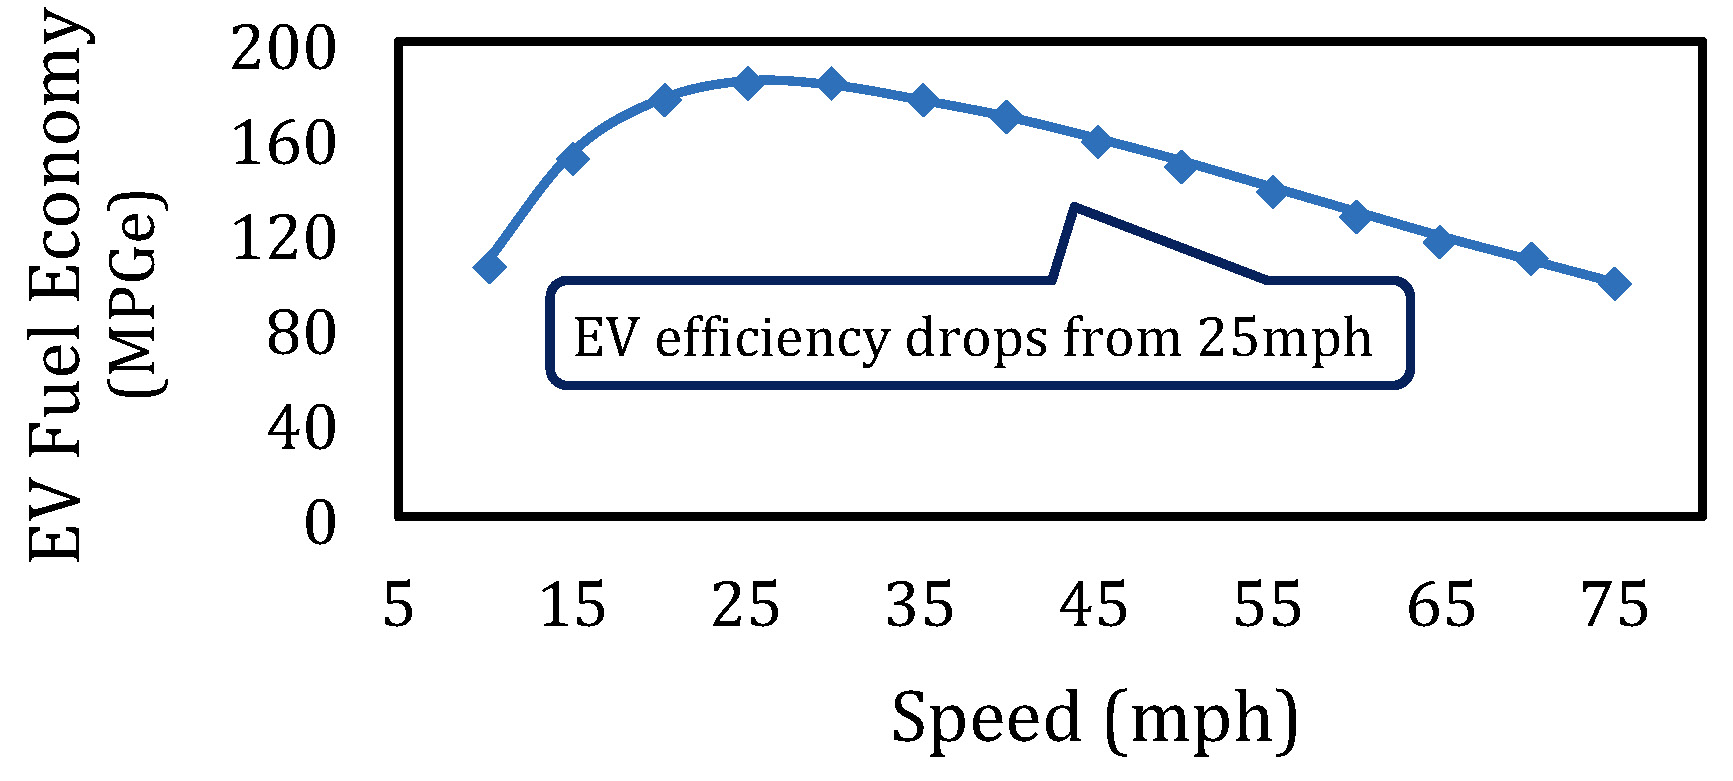
\includegraphics[width=0.8\hsize]{Figures/Al_Faruque/AF_figure1.jpeg}
\caption{Electric vehicle fuel economy for different driving speeds~\cite{AF_11,AF_10}.}
\label{AF_image1}
\end{figure}      

Therefore, modeling and estimation of the driving profile not only help in estimating the driving habits of the drivers, but also enable the designers and engineers to model, estimate, and later optimize the propulsion power in electric vehicles as described in Section~\ref{sec:propulsion}. On the other hand, adjusting and optimizing the driving profile itself is another effective approach to extending the driving range and battery lifetime~\cite{AF_11}. 


%%%%%%%%%%%%%%%%%%%%%%%%%%%%%%%%
\subsection{Modeling and Estimation}

As described in Section~\ref{sec:propulsion}, electric motor of an electric vehicle is the main system contributing to the total power consumption and generation. One of the main factors deciding this propulsion power request, is the driving behavior. The driving behavior is modeled by the values of the driving speed, acceleration, and deceleration at each time instance of the driving route. This model that is called driving profile depends on various parameters of driving such as route conditions and the driver characteristics~\cite{AF_1,AF_17}.

The driving profile can be generated based on the data gathered from one driver while driving, in order to model a driver-specific driving profile; this can be achieved by monitoring multiple state variables of the electric vehicle at runtime using an On Board Diagnosis (OBD) device~\cite{AF_18}. For instance, a biometric system may be incorporated into vehicle security in order to identify the driver. In other words, the amount of pressure a driver applies on the accelerator and brake pedals may be utilized in modeling their driving behavior and personal identification~\cite{AF_19,AF_20}. Moreover, the anger and emotional aggressiveness of the driver may influence its driving behavior~\cite{AF_21,AF_22,AF_23}. Hence, researchers attempt to model these factors that define the driving profile so that they can analyze their influence. Moreover, the safety and energy consumption of the vehicle are important factors influenced by the driving behavior that need to be predicted~\cite{AF_23,AF_24}. 

On the other hand, the driving profile can also be generated based on the gathered data from all the drivers driving on a specific route, in order to model a route-specific driving profile. Certain navigation system databases like Google Maps~\cite{AF_25} generate these models as part of the traffic information of their map databases by gathering data from all their clients or the sensors implemented in the city roads. Moreover, the data of this generic driving behavior can be used to generate driving test cycles. The automotive manufacturers may use these driving cycles to test and analyze the performance of their vehicles in terms of energy consumption and emissions~\cite{AF_26,AF_27}.

In summary, these driving profile models can be used for the purpose of personal identification, driver characteristics estimation, or estimation of the propulsion power by the electric motor. Later on, they can be adjusted and optimized for a specific driver or driving route in order to improve the performance of the electric vehicle in terms of battery lifetime, driving range, or even safety.

Typically, driving profile can be implemented simply as a matrix representing consecutive segments of the driving route ($\bar{s}$)~\eqref{AF_eq1}. Each row in the matrix stores the information of the route condition and the corresponding driver reactions for each segment of the driving route.

\begin{equation}
%\[
\bar{s} = 
\begin{bmatrix} 	
time 		& length 	& speed 	& acceleration 	& slope \\ 
t_1		&l_1		&v_1		&a_1			&\alpha_1	\\
\vdots 	&\vdots 	&\vdots 	&\vdots 		&\vdots \\
t_n		&l_n		&v_n		&a_n			&\alpha_n	
\end{bmatrix}
\label{AF_eq1}
%\]
\end{equation}

The information for each segment may contain the average time taken to drive the segment ($t_i$); segment length ($l_i$); average vehicle speed ($v_i$); average vehicle acceleration ($a_i$); and road slope ($\alpha_i$).
The values for these elements can be retrieved based on the data gathered for the drivers and map databases as explained above~\cite{AF_1,AF_11}.


%%%%%%%%%%%%%%%%%%%%%%%%%%%%%%%%
\subsection{Runtime Driving Management and Power Optimization}

Driving management and route optimization have always been the most common problem of vehicles to improve the quality of transportation. Typically, driving management methodologies consider the driving distance and the driving time in order to find the fastest and shortest route to a specific destination~\cite{AF_37,AF_38,AF_39}. Map databases are utilized to provide the required information for selecting the optimal route. More detailed driving profile modeling can enable the methodologies to optimize the driving routes considering other objectives such as energy consumption and the battery lifetime. For instance, driving profile model containing the segment information such as road slope and average speed will enable the driving management methodology to estimate the energy consumption of the electric motor at each segment. The routing algorithm can be implemented such that the weights for the edges of the graph are defined as same as the objective considered in the driving management as shown in Fig.~\ref{AF_image3}~\cite{AF_40,AF_41,AF_42}. 

\begin{figure}
\centering
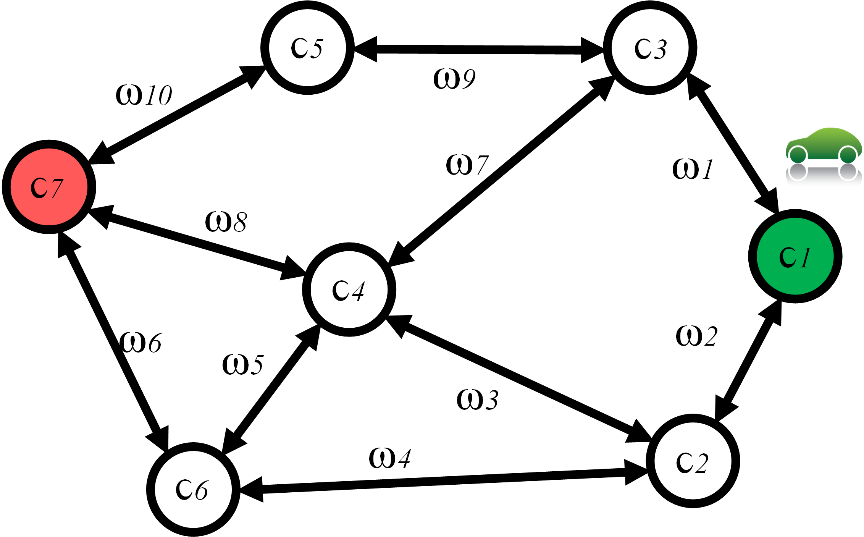
\includegraphics[width=0.8\hsize]{Figures/Al_Faruque/AF_figure3.png}
\caption{Routing problem labeled with edge weights~\cite{AF_11}.}
\label{AF_image3}
\end{figure}      

The results have shown that by sacrificing about 3 minutes of the driving time, a driving management can take a detailed driving profile and propulsion power modeling into account and reduce the energy consumption by 11.9\% compared to the fastest route~\cite{AF_11,AF_17}.

Moreover, vehicles implement energy management methodologies that utilize the driving profile modeling to improve the driving range by reducing the energy consumption. For instance, the power split among the battery, combustion engine, and ultracapacitor is very important to the performance of the vehicle and its driving range. Predictive models of the driving profile are incorporated in the control to facilitate with the system estimation and control optimization~\cite{Park:DAC13,AF_8,AF_10,AF_34,AF_35,AF_36}.


%%%%%%%%%%%%%%%%%%%%%%%%%%%%%%%%
\section{Non-Propulsion Power Modeling, Estimation, and Runtime Optimization} \label{sec:non-propulsion}
%%%%%%%%%%%%%%%%%%%%%%%%%%%%%%%%

%%%%%%%%%%%%%%%%%%%%%%%%%%%%%%%%
Besides electric motors, auxiliary systems in electric vehicles are the other major systems which influence its power consumption. Non-propulsion power requested by the auxiliary systems mostly depend on the functionality and objective of the system regardless of the driving behavior and profile. For instance, Heating, Ventilation, and Air Conditioning (HVAC) as an auxiliary system is responsible to maintain the cabin temperature in a comfort thermal range for the passengers~\cite{AF_13,AF_14,AF_15,AF_16}.

\begin{figure}
\centering
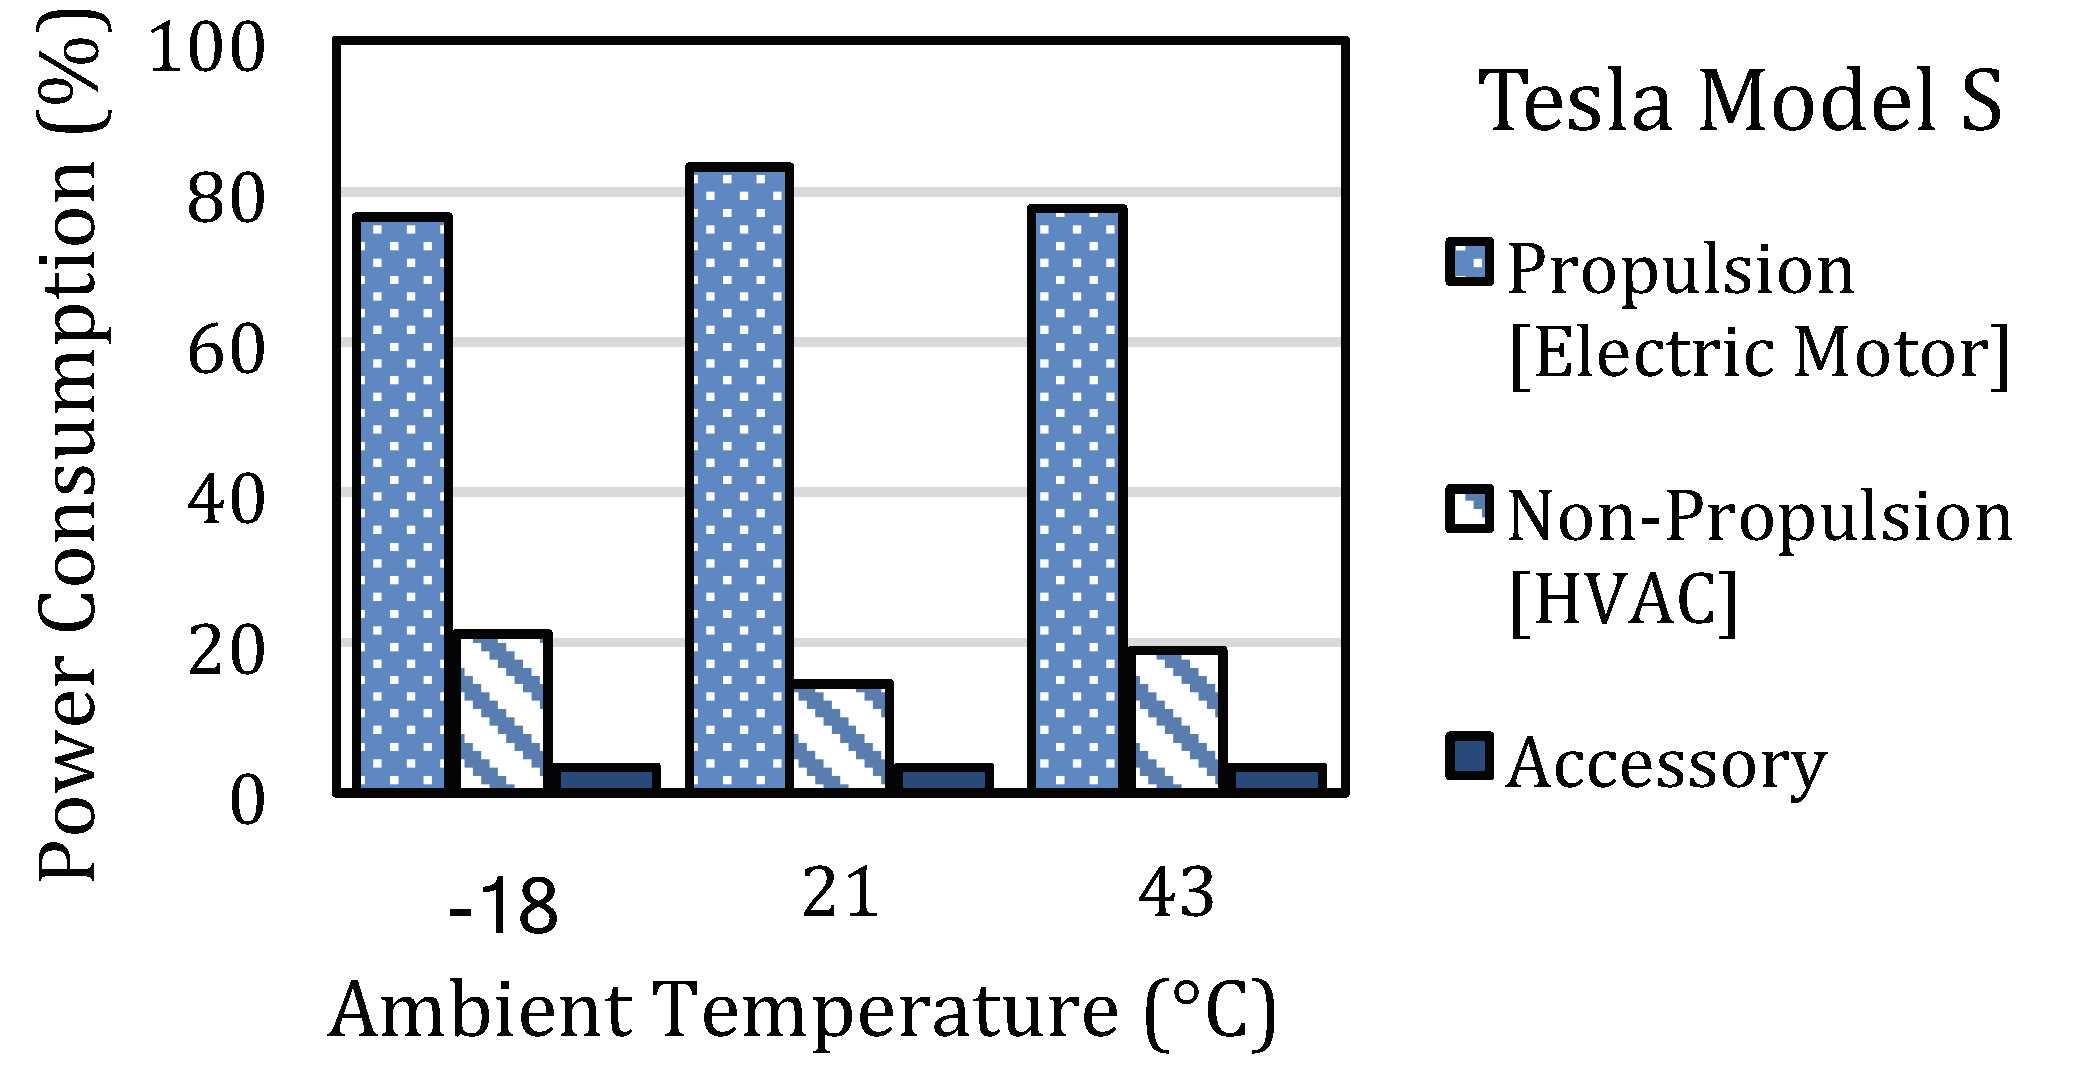
\includegraphics[width=0.8\hsize]{Figures/Al_Faruque/AF_figure2.jpeg}
\caption{Percentages of three types of power consumption in an electric vehicle for different ambient temperatures~\cite{AF_1,AF_10}.}
\label{AF_image2}
\end{figure}      

Fig.~\ref{AF_image2} illustrates the details of three types of power consumption: 1) propulsion, 2) non-propulsion, and 3) accessory power consumption, for different temperatures in a Tesla Model~S. The fraction of the HVAC power consumption (non-propulsion) mainly depends on the ambient temperature and the required comfort range. Although HVAC energy is proportional to the driving time, it is not sensitive to the detailed driving profile (speed and acceleration) unlike the electric motor. This characteristic shows that auxiliary systems have flexible load and power pattern. Hence, modeling and estimation of the auxiliary systems such as HVAC will enable the electric vehicle designers and engineers to further exploit this characteristic. Therefore, they will be able to adjust and optimize the non-propulsion power, e.g. HVAC power, in order to improve the operating parameters of the electric vehicles such as driving range and battery lifetime.


%%%%%%%%%%%%%%%%%%%%%%%%%%%%%%%%
\subsection{Modeling and Estimation}

Overall, the amount of non-propulsion power requested in an electric vehicle depends on the targeted auxiliary systems, their functioning components and the control process implemented to integrate and manage them.
For instance, an HVAC is controlled by an automotive climate control in order to maintain the cabin temperature ($T_z$). The cabin temperature is influenced by the supply air ($T_s$) to the cabin and other thermal loads including the heat exchange with outside and the solar radiation. The air supply temperature is controlled by adjusting the temperature set points on heating and cooling coils. Moreover, variable air valves are utilized in a more complex HVAC in order to maintain the required thermal comfort for the passengers even in a multi-zone cabin. These systems utilize variable-speed fans and air ducts to provide the supply air to the zone(s).

Typically, the power consumption of the cooling ($P_c$) and heating coils ($P_h$) depends on the energy difference between their inlet and outlet air flows. Moreover, the power consumption of the variable-speed fans ($P_f$) is quadratically related to the air flow rate ($\dot{m}_z$). The thermodynamics of the cabin temperature considering all the control inputs and variables are modeled by energy balance differential equations. Hence, Ordinary Differential Equations (ODE) can be implemented to model and estimate the thermodynamic behavior of the HVAC system and its the instantaneous power consumption. 

These models are typically used for evaluating and analyzing the performance of the auxiliary system – HVAC – and its influence on the whole vehicle. For instance, the researchers estimate the energy consumption of the HVAC system regarding different driving conditions like weather. This estimation is leveraged in order to predict the driving range of the vehicle and analyze how much HVAC influence this crucial parameter of the vehicle~\cite{AF_23,AF_28,AF_29}. 

%%%%%%%%%%%%%%%%%%%%%%%%%%%%%%%%
\subsection{Runtime Control Scheduling}

During the operation of an electric vehicle, there are multiple control inputs which can be adjusted and optimized towards a certain objective. The controllers implemented are responsible to monitor the state variables and decide these control inputs. They may utilize the integrated modeling towards their estimation and optimization purpose. Previously in Sections~\ref{sec:propulsion} and \ref{sec:driving_profile}, we discussed how modeling of propulsion power and driving profile may help in optimizing the vehicle speed, acceleration, driving route, and power split.

Auxiliary systems in electric vehicles implement control algorithms responsible for scheduling control actions in their systems. The decisions made by the controller will influence the non-propulsion power requested by the auxiliary systems. For instance, in an auxiliary system like HVAC, an automotive climate control basically senses the cabin temperature and weather and decides how hot and cool the supply air temperature should be, given the model of the cabin and HVAC~\cite{AF_30,AF_31,AF_32,AF_33}.

The automotive climate control adjusts the control inputs into the HVAC in order to maintain the cabin temperature around a certain target and within a comfort range. The climate control may be implemented using an MPC or a rule-based control. The controller may leverage the HVAC dynamic and non-propulsion power models to estimate the state, auxiliary, and output variables according to specific control inputs for a certain prediction horizon in the future. The controller utilizes an optimizer to adjust the control inputs such as heating and cooling coil temperature set points and the fan speed of the prediction horizon while considering the constraints. The controller may be responsible to minimize an objective or cost function.

An automotive climate control may only consider the cabin temperature as the objective~\cite{AF_30,AF_31,AF_32,AF_33}. However, the power consumption of the HVAC (non-propulsion) and the electric motor (propulsion) may be considered as well in order to reduce the influence on the electric vehicle energy and battery capacity loss~\cite{AF_10,AF_29}. Therefore, depending on the details of the modeling, the cost function may include the 1) cabin temperature variation, 2) HVAC energy consumption, and 3) battery capacity loss. Moreover, there are certain constraints on the control inputs and state variables which should be satisfied during the optimization and control process.

Therefore, the control scheduling of the auxiliary systems may reduce the battery stress, improve the driving range, and the battery lifetime by adjusting the non-propulsion power such that it compensates for the propulsion power or the quality of the system. It has been shown that an MPC-based methodology given the models is able to minimize the non-propulsion power on average 39\% compared to the fuzzy-based methodology which minimizes by 6\%~\cite{AF_10,AF_32,AF_43}.


